\section*{Appendix A - Ábrák} \label{A}
\topskip0pt
\vspace*{\fill}
\begin{center}
    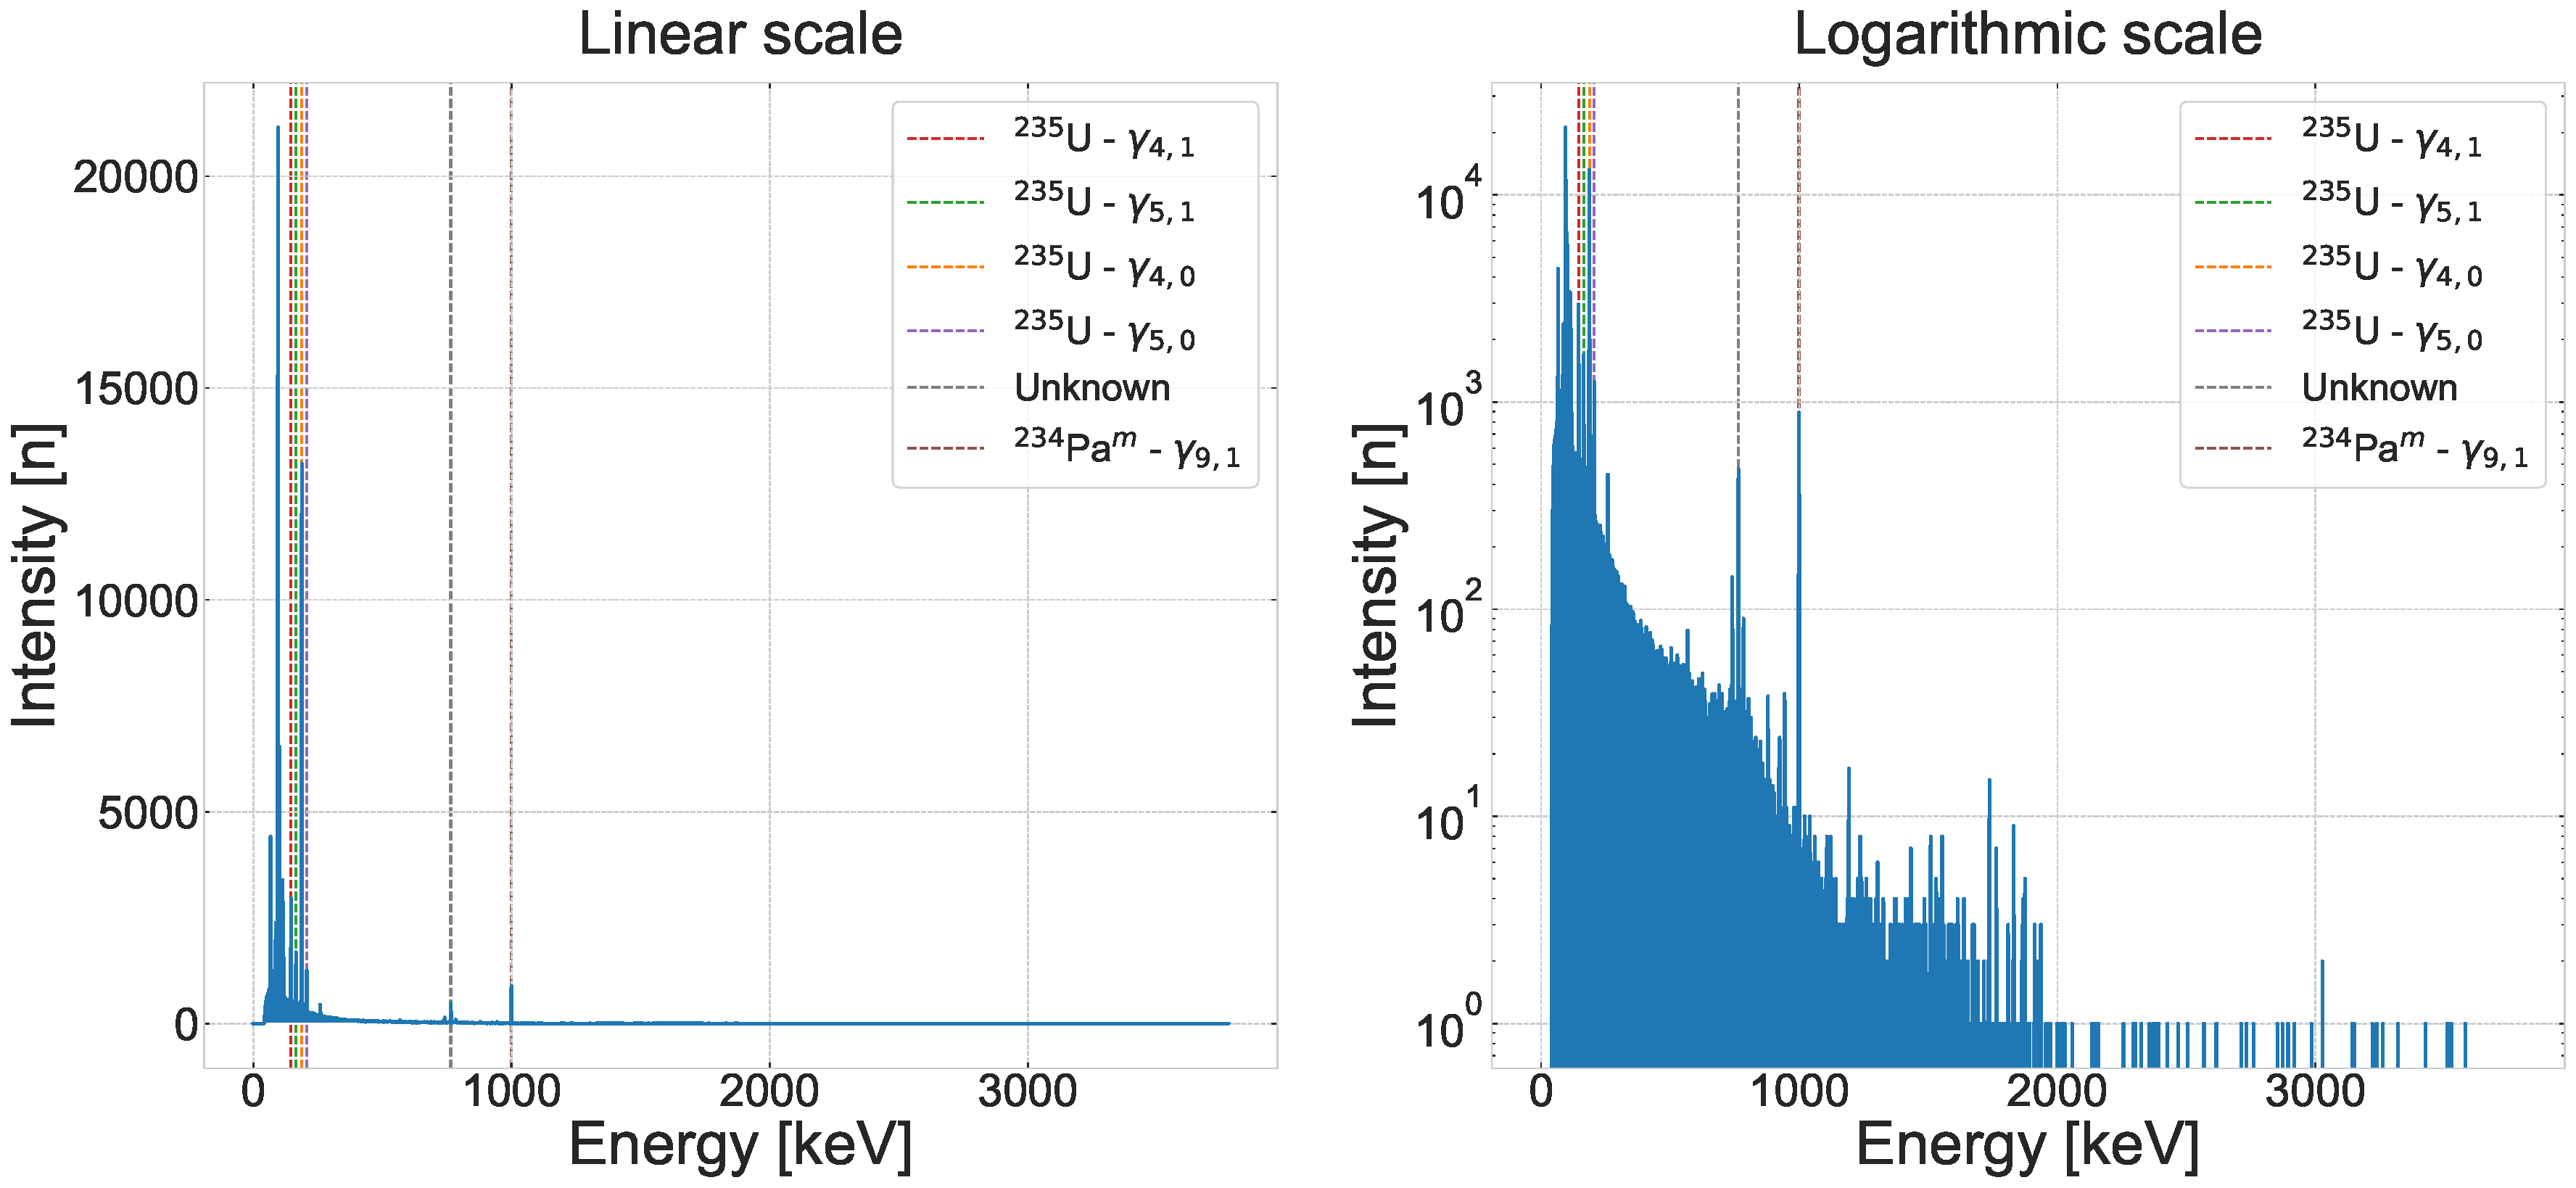
\includegraphics[width=\textwidth]{{images/full_spectra}.pdf}
    \captionof{figure}{Az általam vizsgált anyag teljes lemért gamma-spektruma. Az egyes karakterisztikus csúcsok színes, szaggatott vonallal vannak jelölve.} \label{fig:1}
\end{center}
\begin{center}
    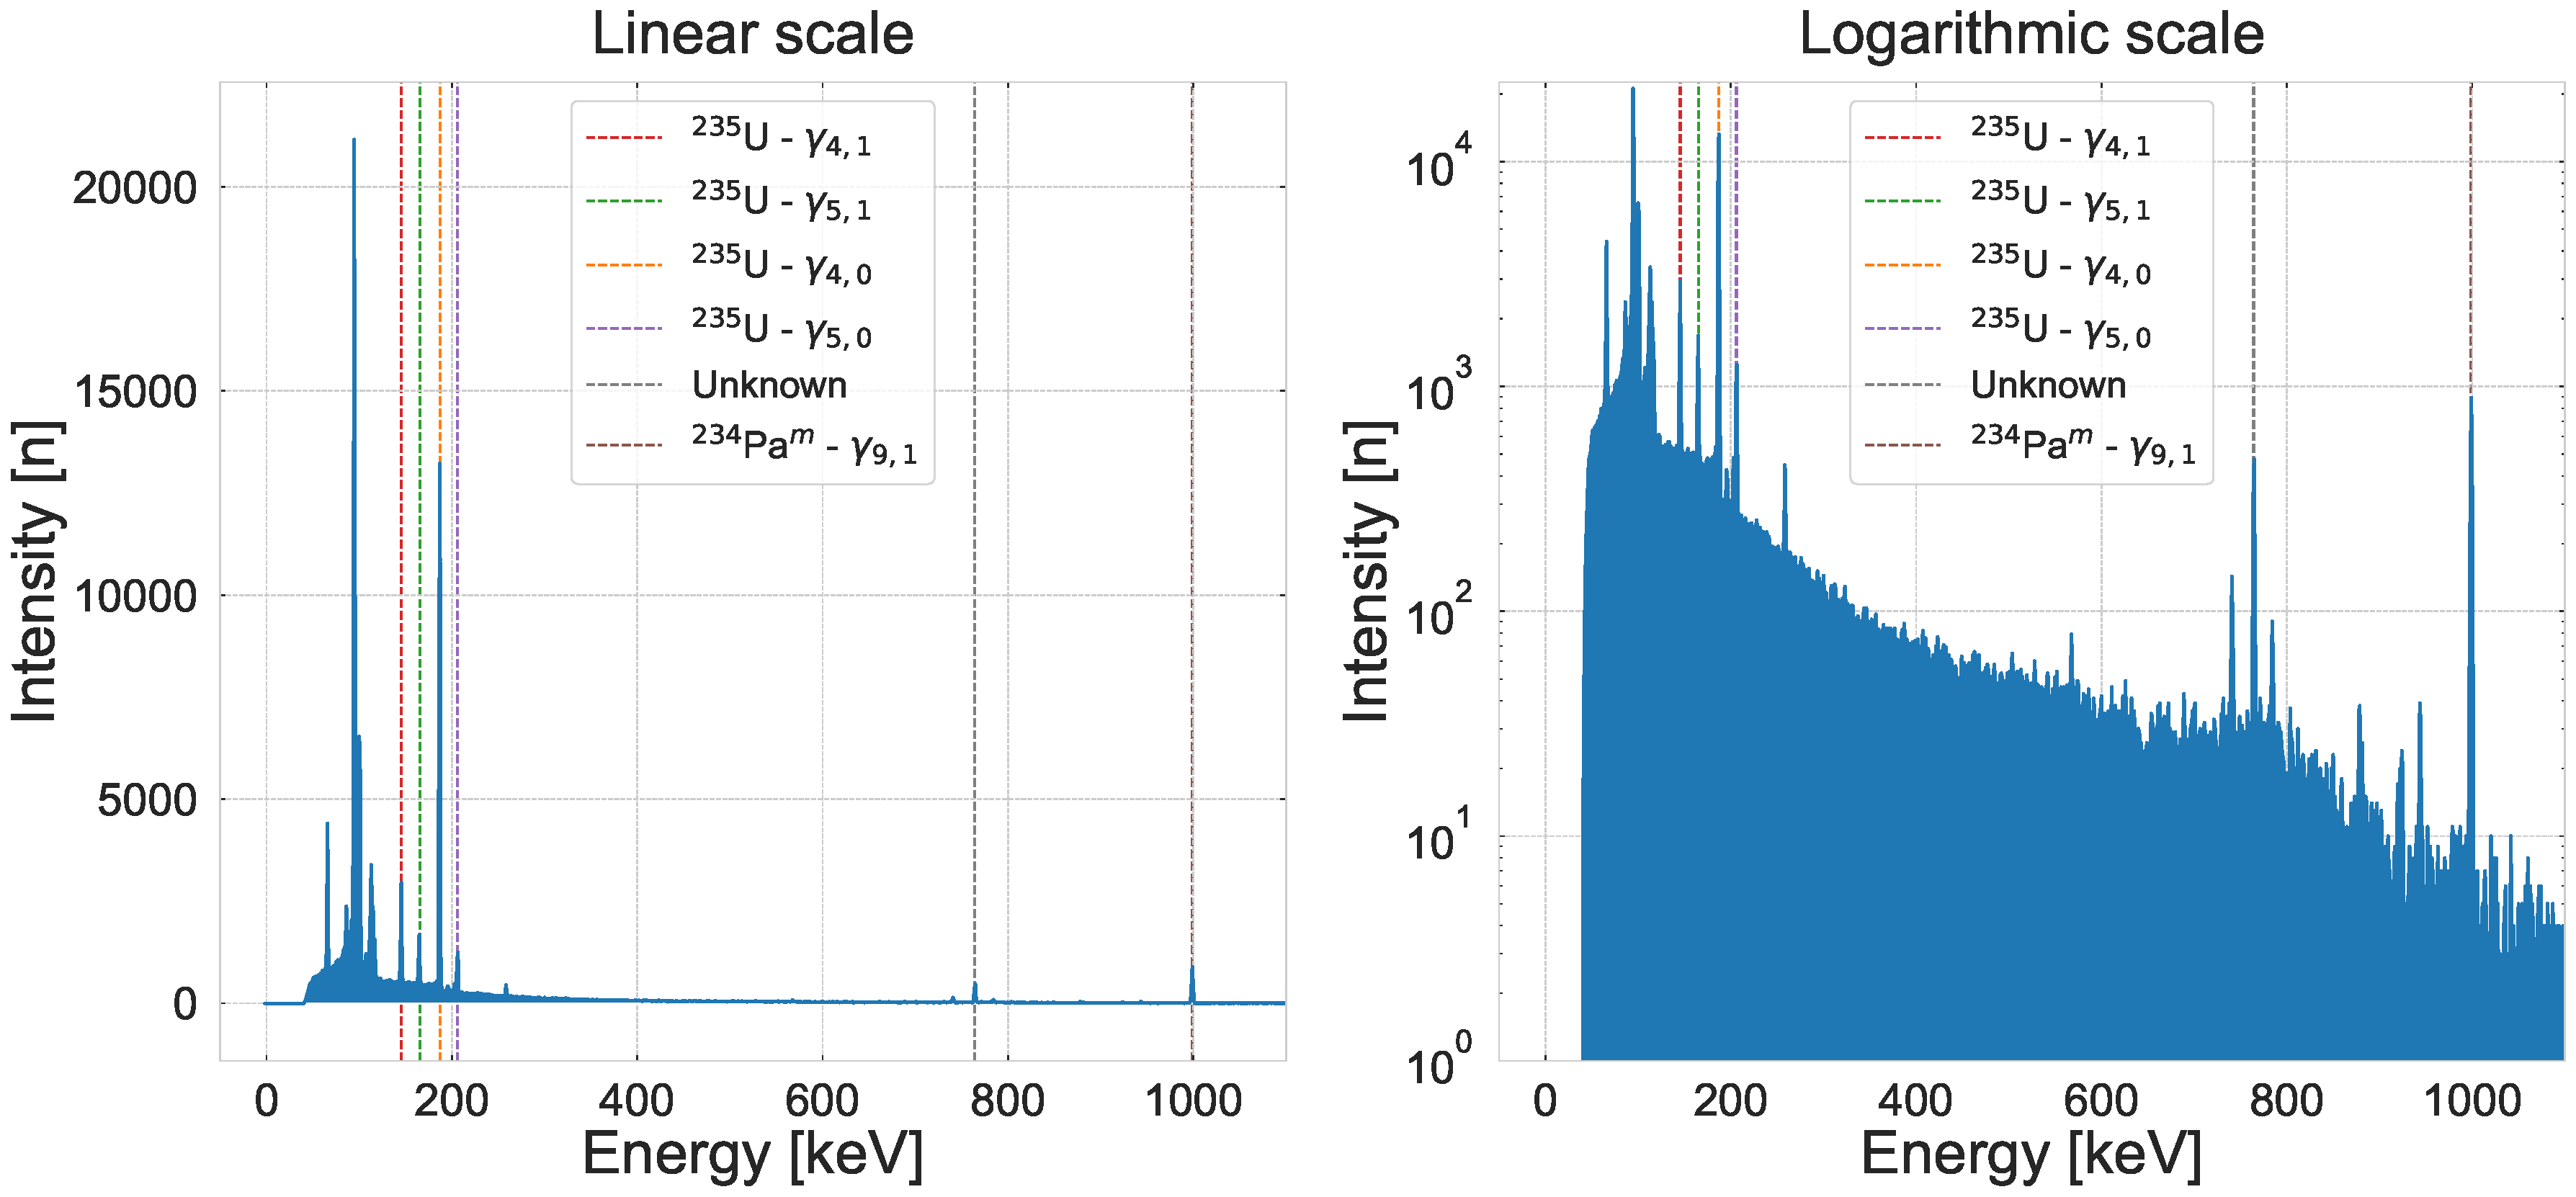
\includegraphics[width=\textwidth]{{images/spectra_lims_-50.00_1100.00_full_height}.pdf}
    \captionof{figure}{Az általam vizsgált anyag gamma-spektruma a $0\ \text{keV} - 1100\ \text{keV}$ intervallumban. Az egyes karakterisztikus csúcsok színes, szaggatott vonallal vannak jelölve.} \label{fig:2}
\end{center}
\begin{center}
    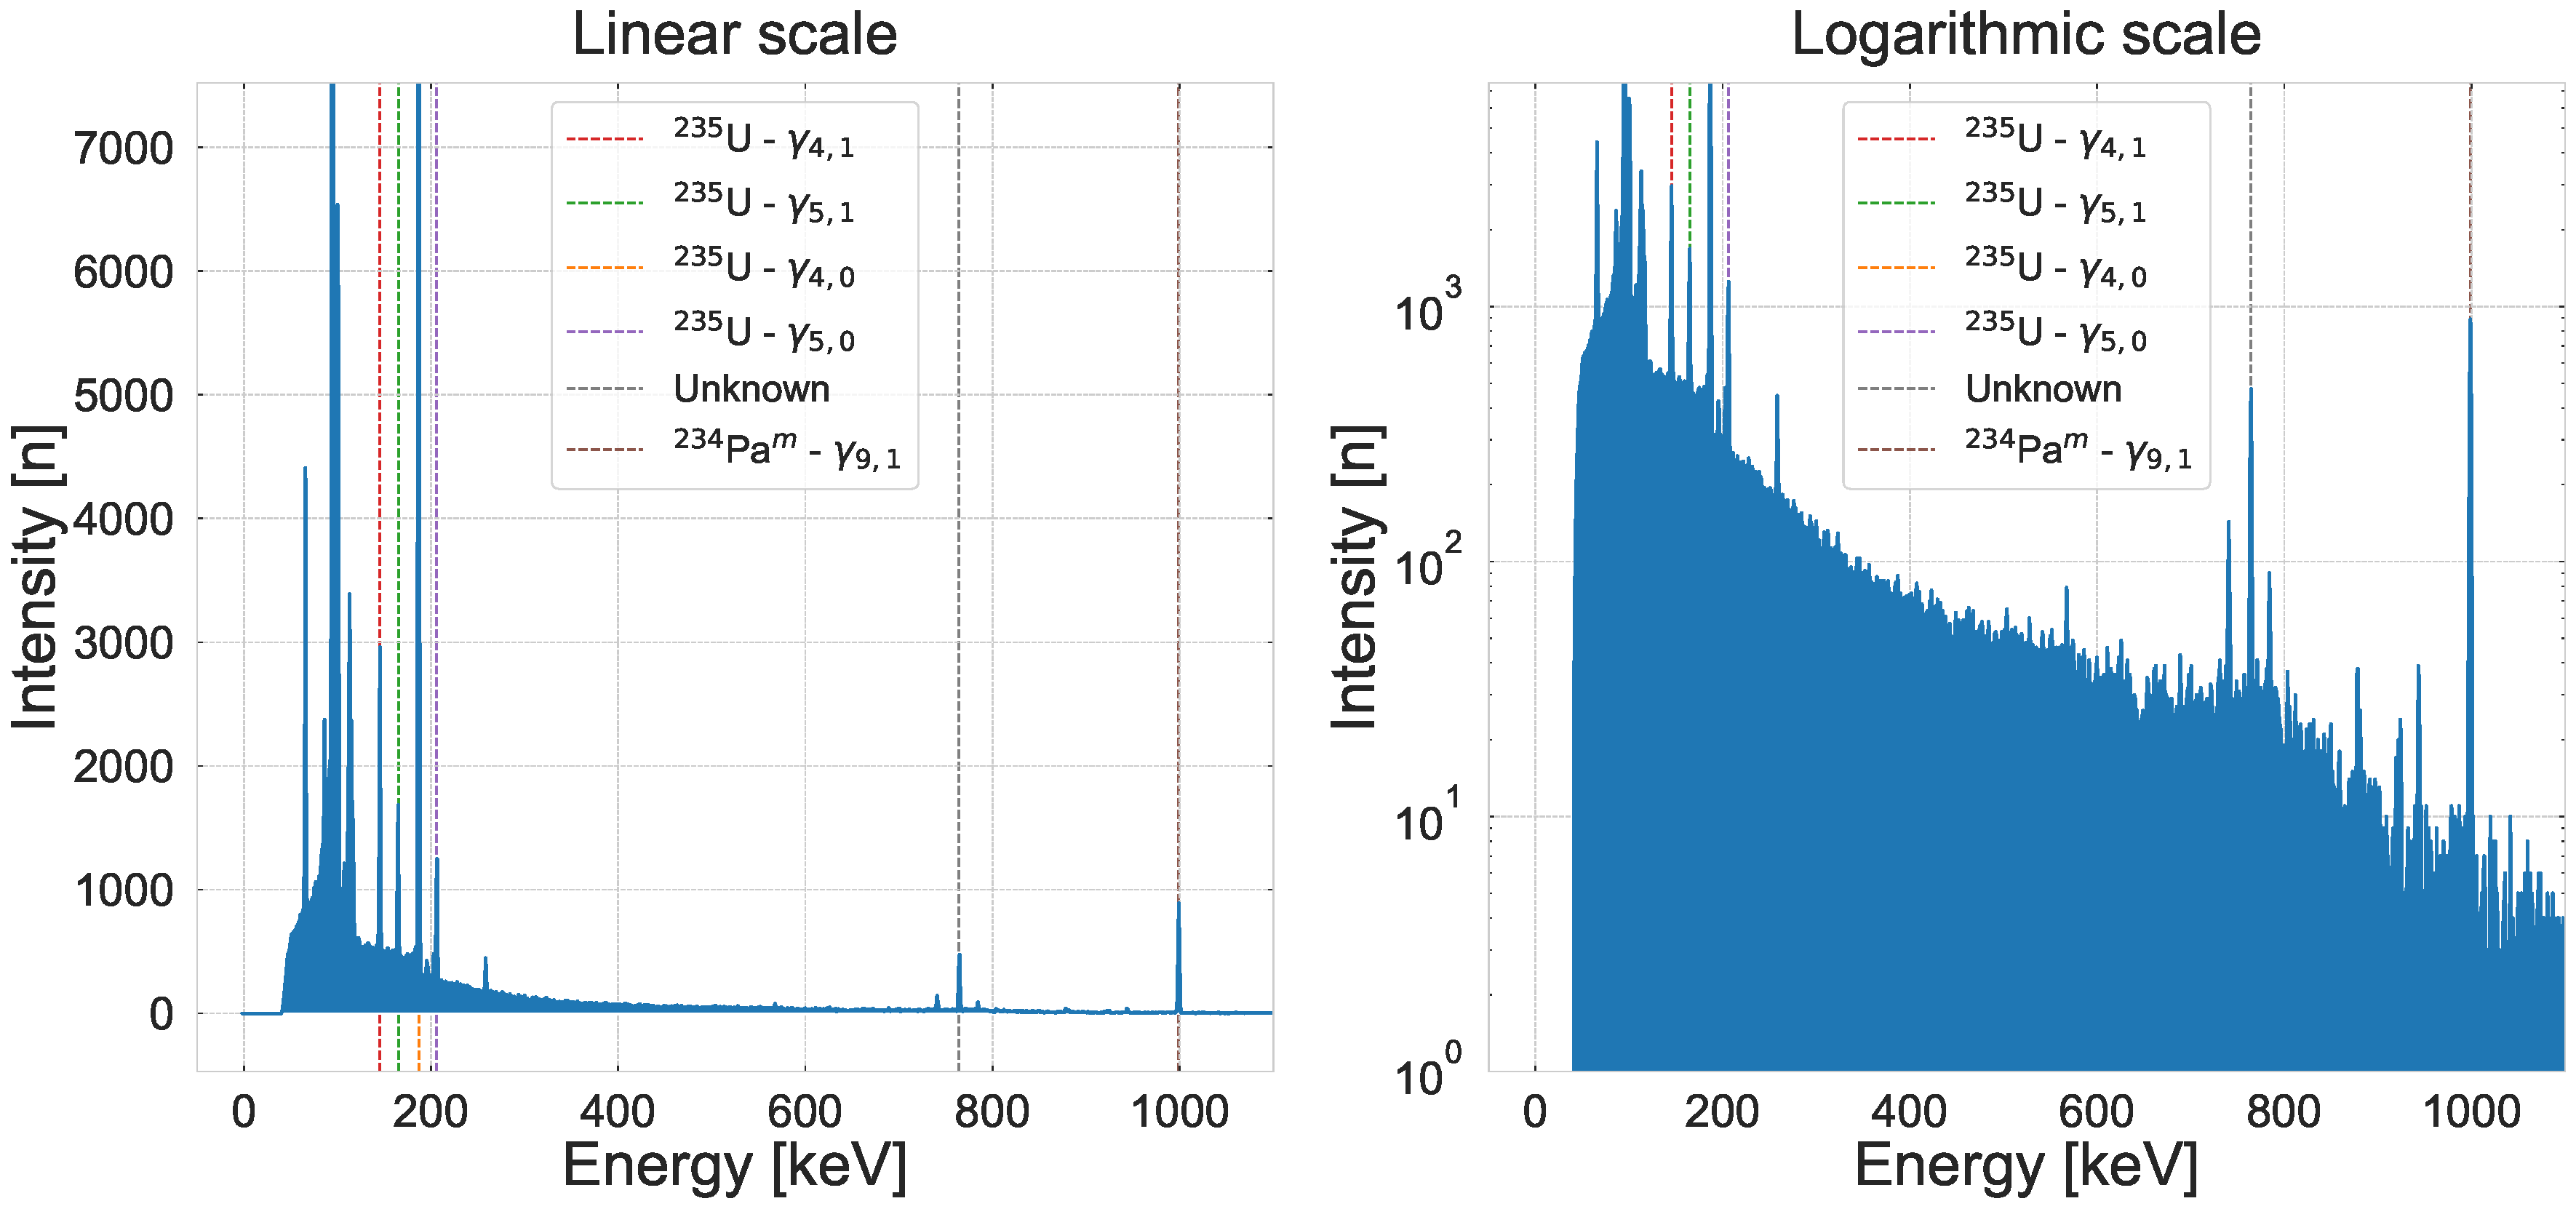
\includegraphics[width=\textwidth]{{images/spectra_lims_-50.00_1100.00_small_height}.pdf}
    \captionof{figure}{Az általam vizsgált anyag gamma-spektruma a $0\ \text{keV} - 1100\ \text{keV}$ intervallumban. Az ábrán a (\ref{fig:2})-es ábrán szereplő $y$-tengely alsó harmada van megjelenítve. Az egyes karakterisztikus csúcsok színes, szaggatott vonallal vannak jelölve.} \label{fig:3}
\end{center}
\vspace*{\fill}
\newpage
\topskip0pt
\vspace*{\fill}
\begin{center}
    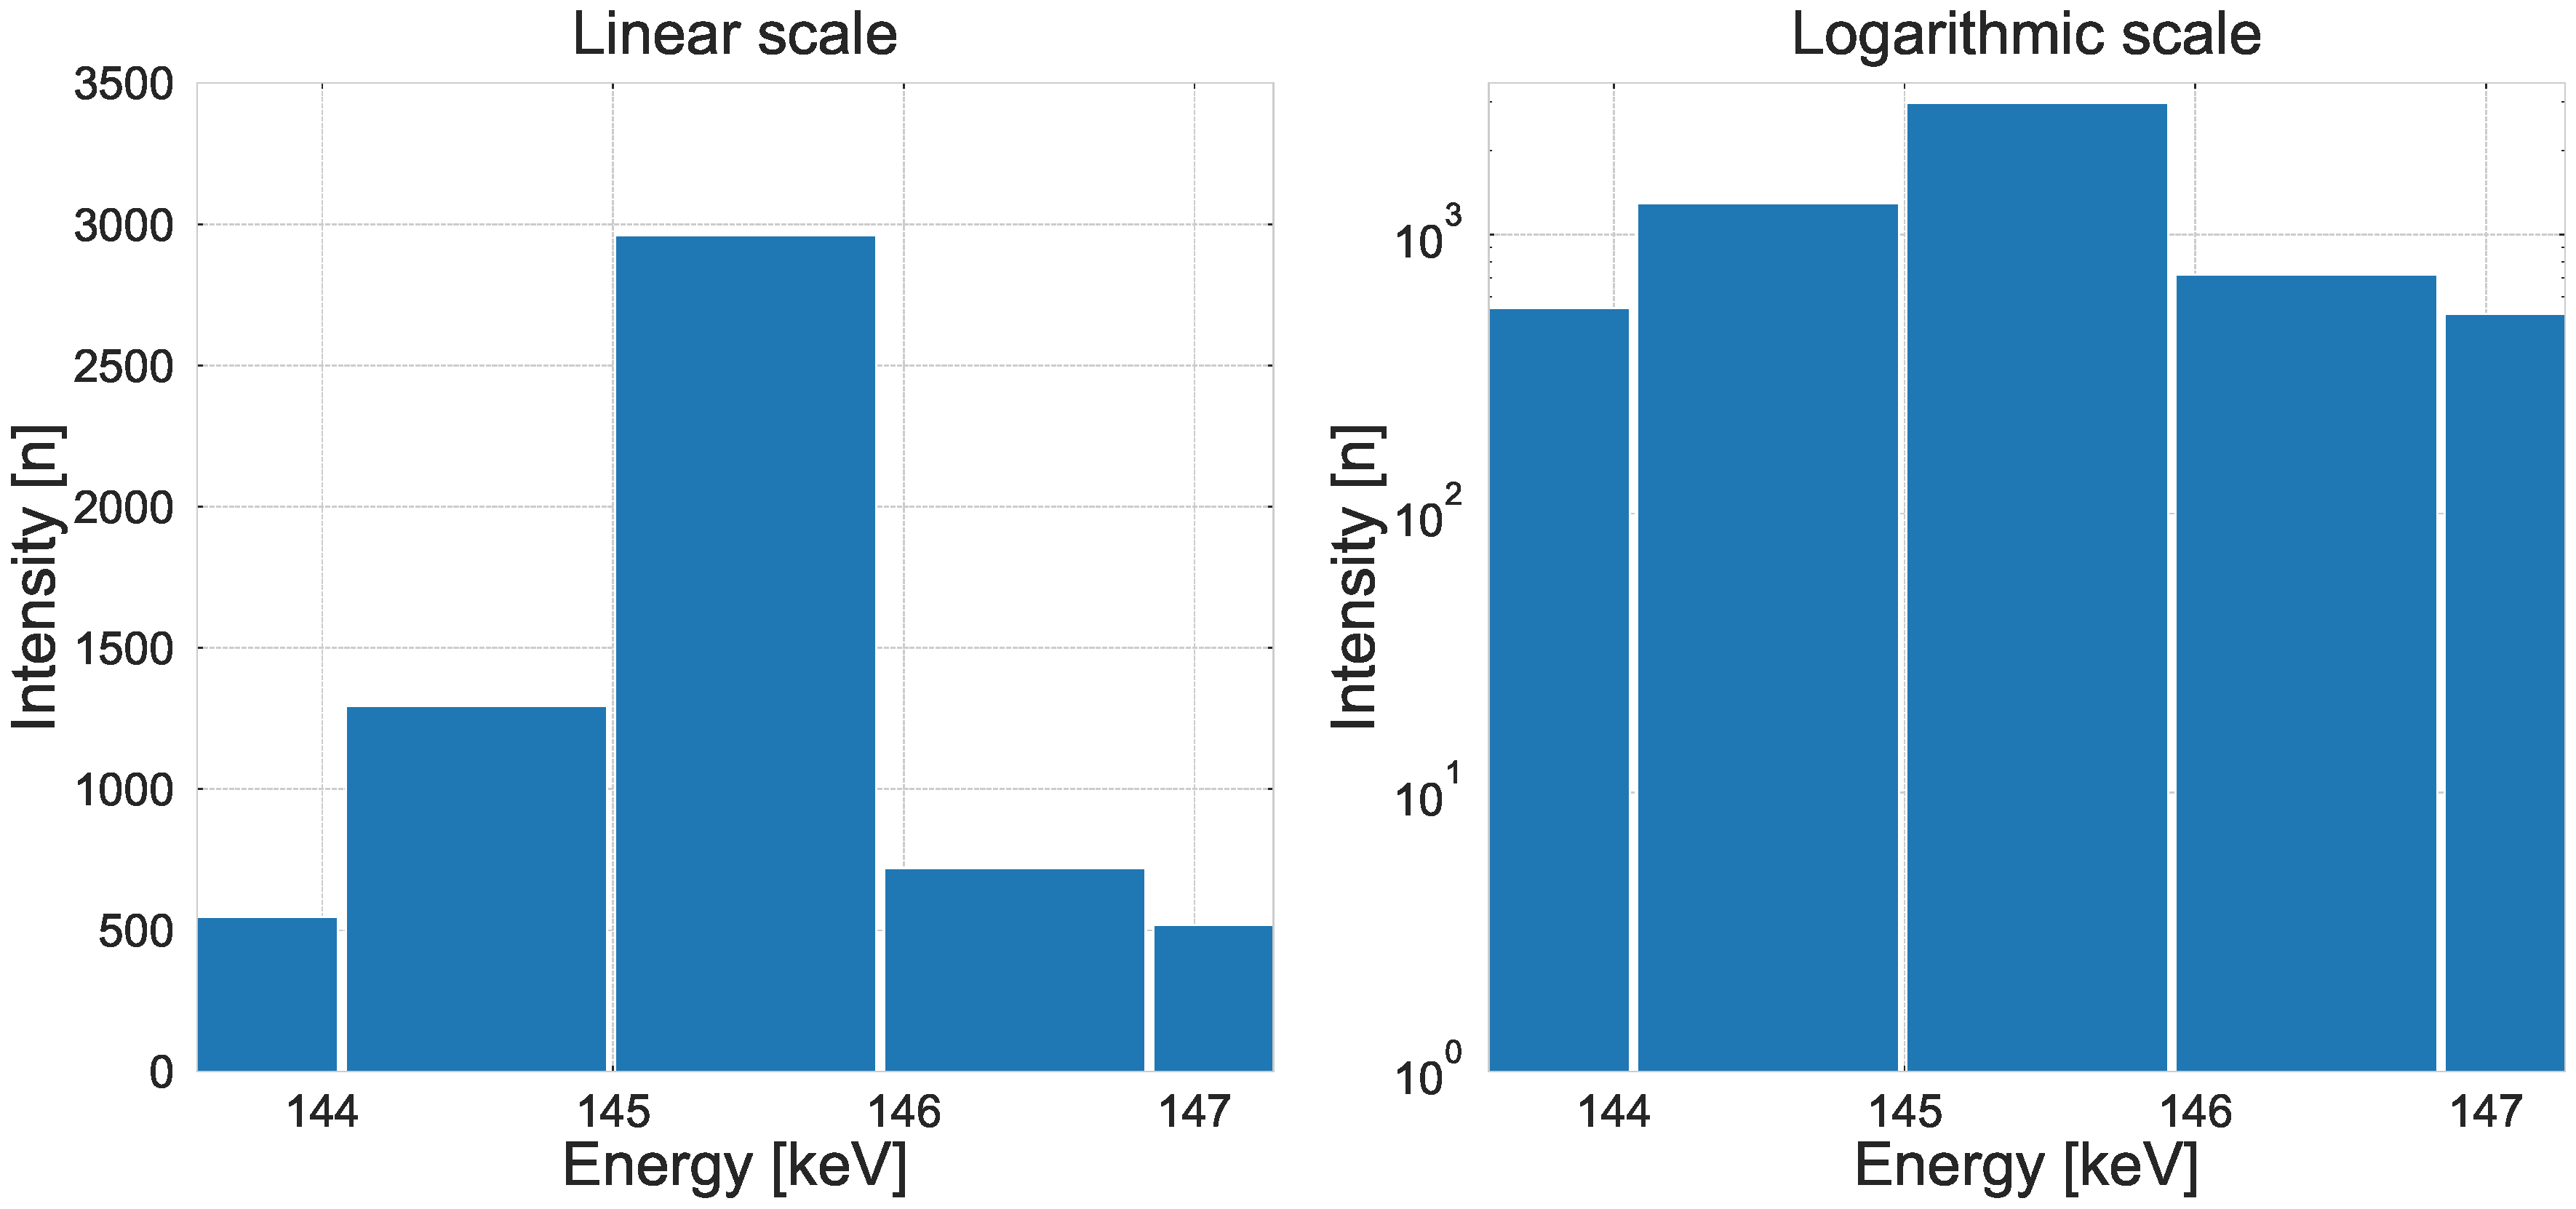
\includegraphics[width=\textwidth]{{images/spectra_lims_143.57_147.27_U235_g4_1}.pdf}
    \captionof{figure}{Az általam vizsgált anyag gamma-spektrumában található $^{235}$U, $\gamma_{4,1}$ tranziensből származó fotonjának foto-csúcsa.} \label{fig:4}
\end{center}
\begin{center}
    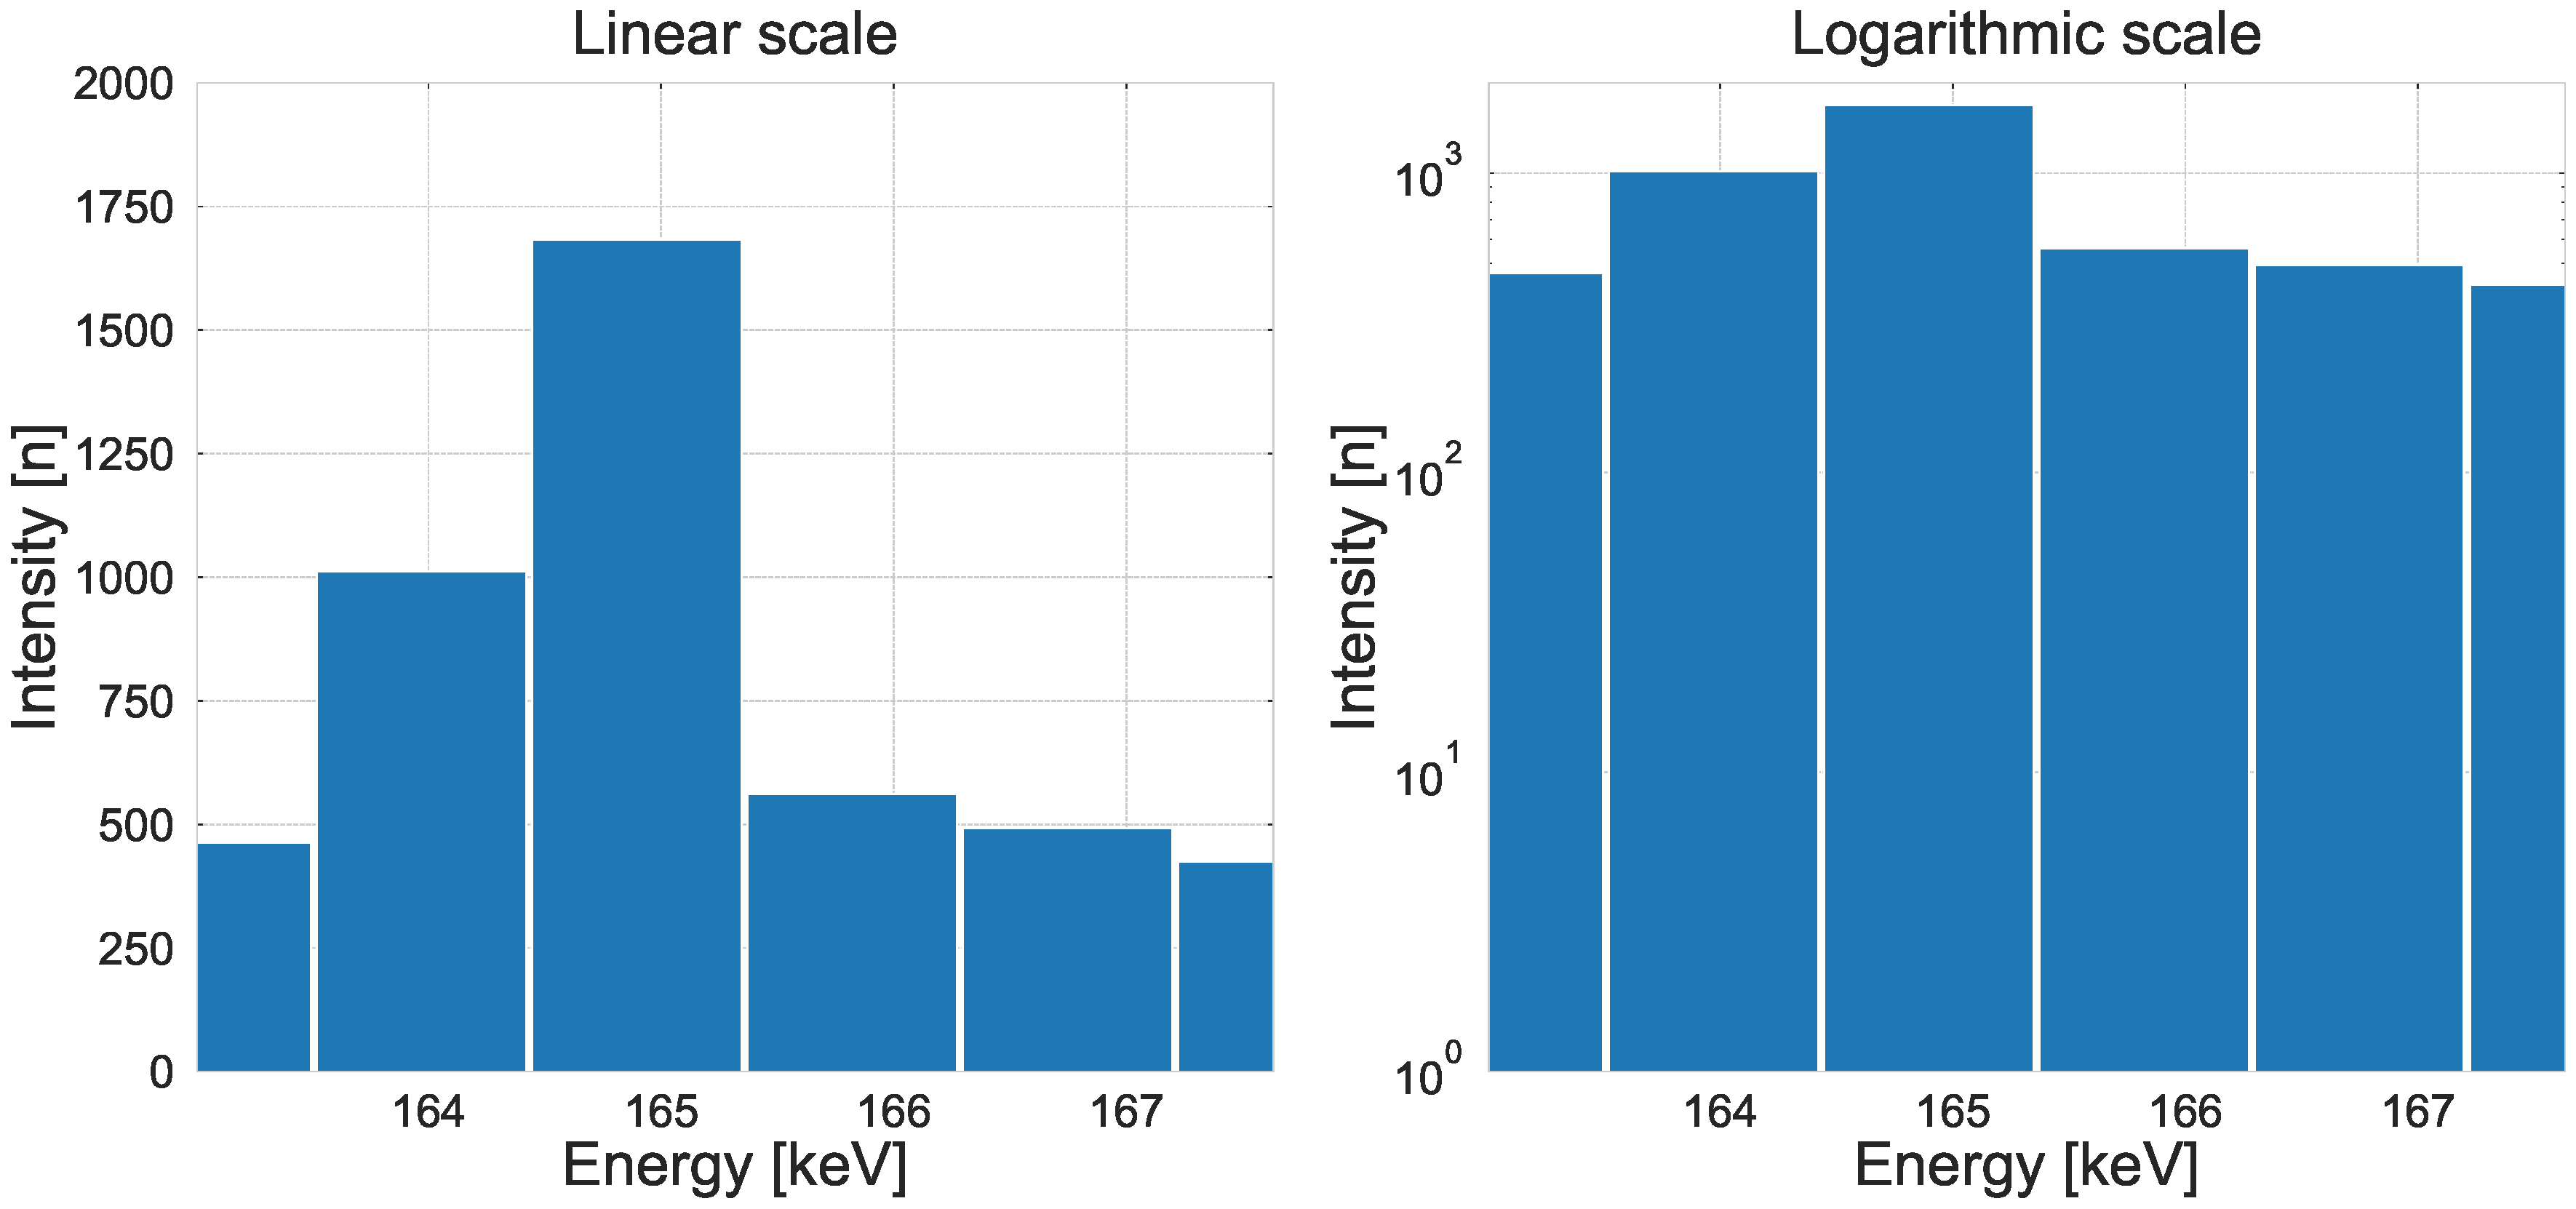
\includegraphics[width=\textwidth]{{images/spectra_lims_163.00_167.63_U235_g5_1}.pdf}
    \captionof{figure}{Az általam vizsgált anyag gamma-spektrumában található $^{235}$U, $\gamma_{5,1}$ tranziensből származó fotonjának foto-csúcsa.} \label{fig:5}
\end{center}
\begin{center}
    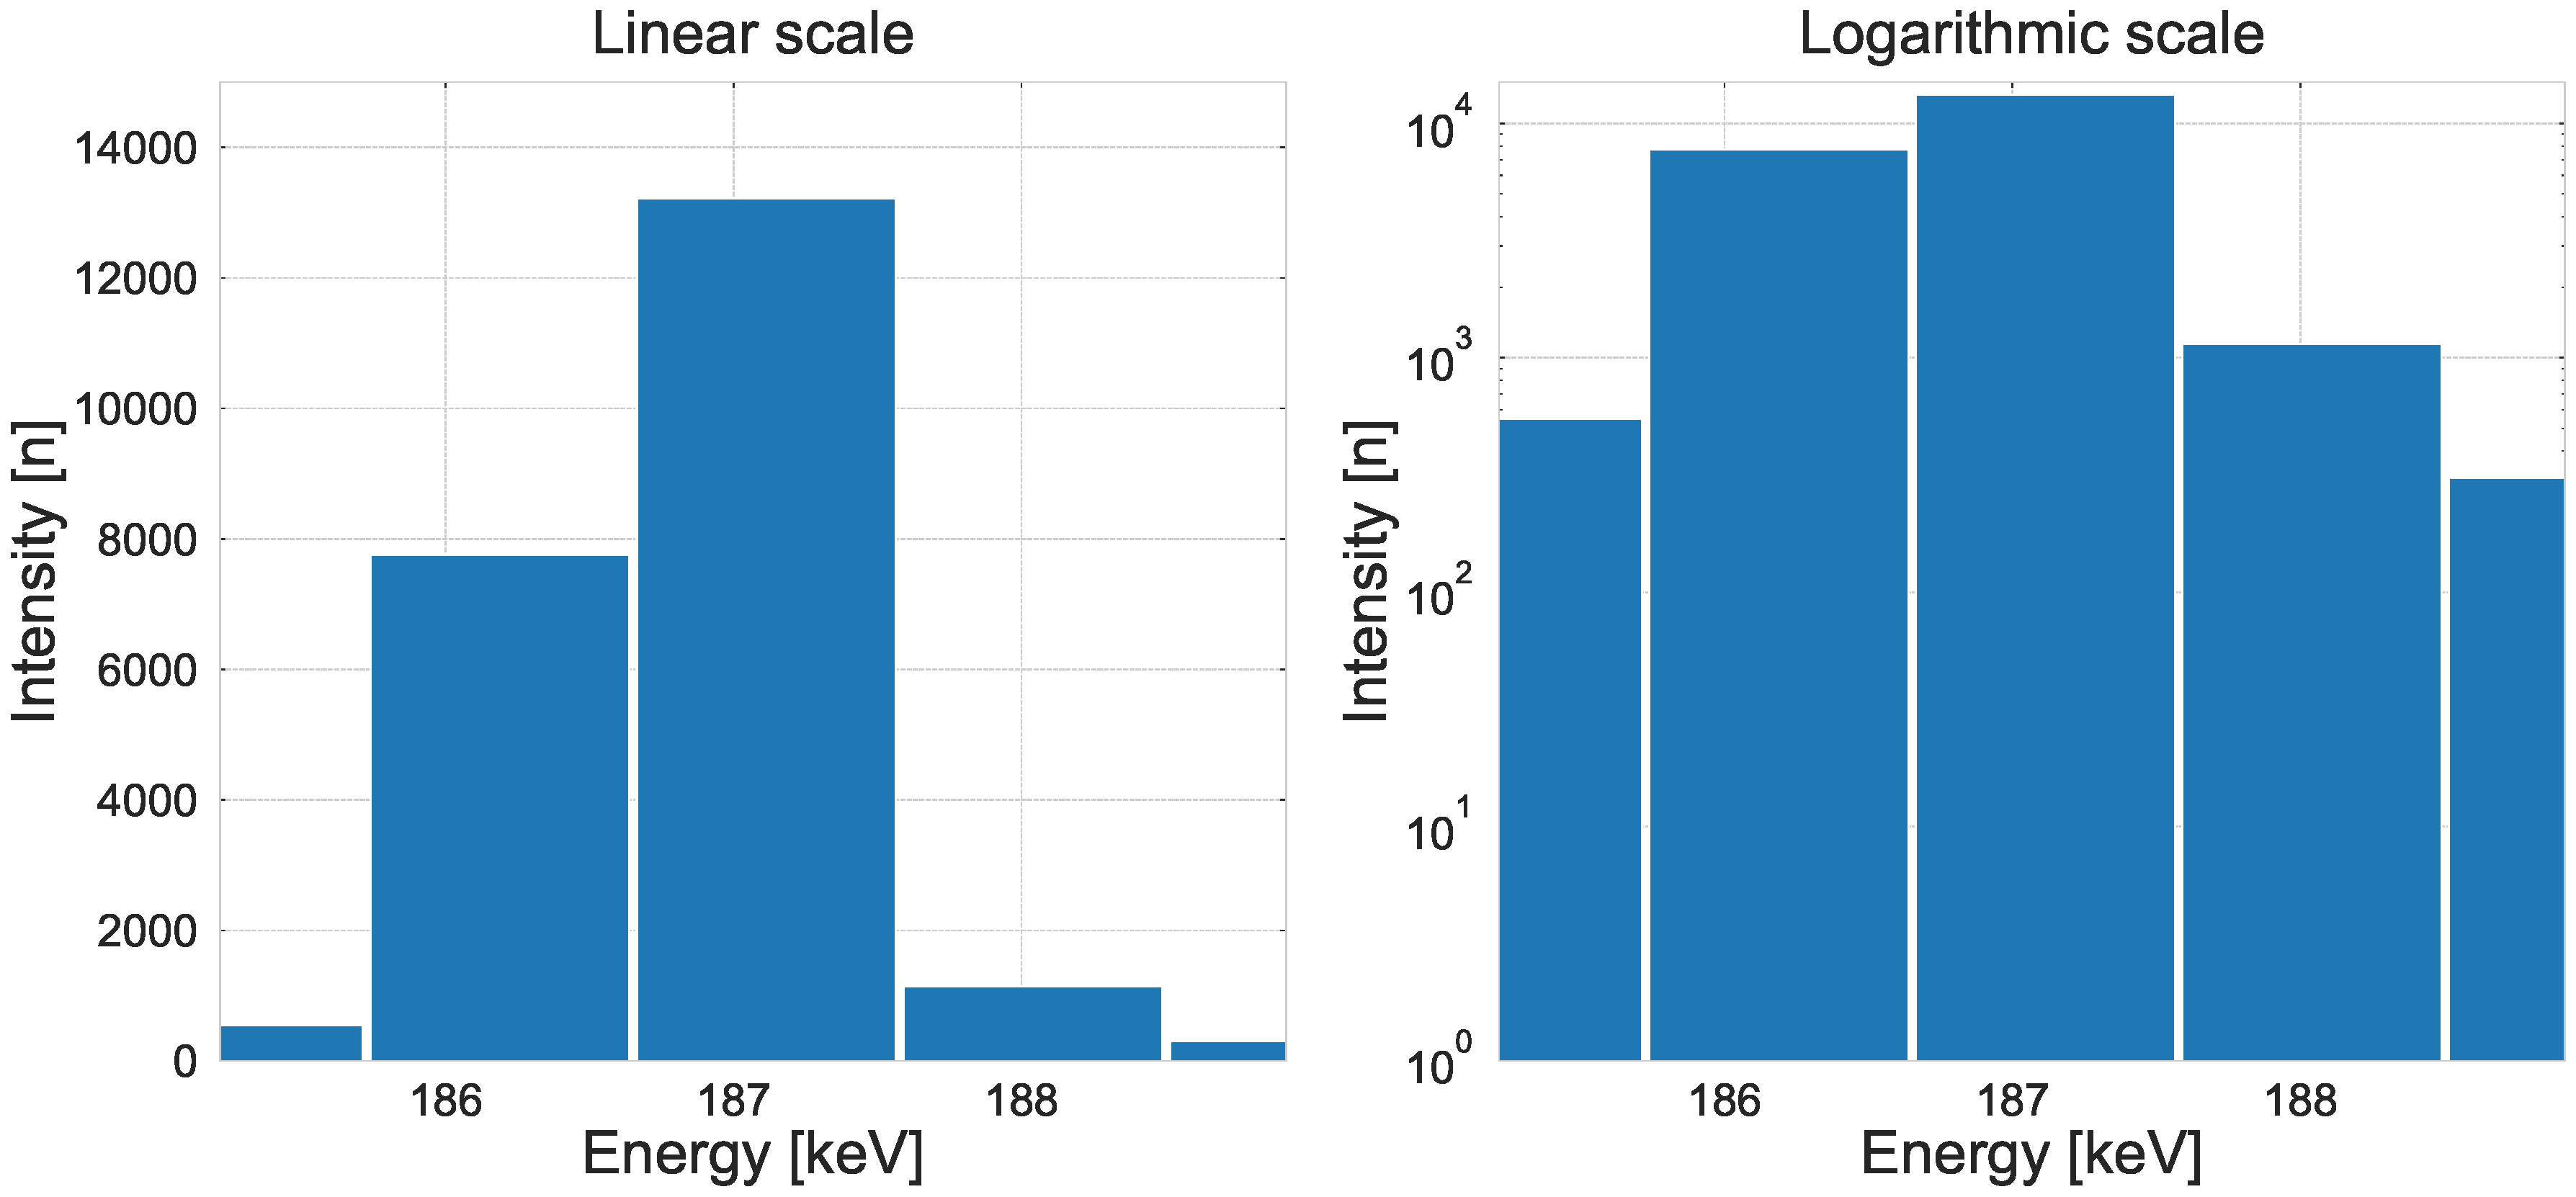
\includegraphics[width=\textwidth]{{images/spectra_lims_185.22_188.92_U235_g4_0}.pdf}
    \captionof{figure}{Az általam vizsgált anyag gamma-spektrumában található $^{235}$U, $\gamma_{4,0}$ tranziensből származó fotonjának foto-csúcsa.} \label{fig:6}
\end{center}
\vspace*{\fill}
\newpage
\topskip0pt
\vspace*{\fill}
\begin{center}
    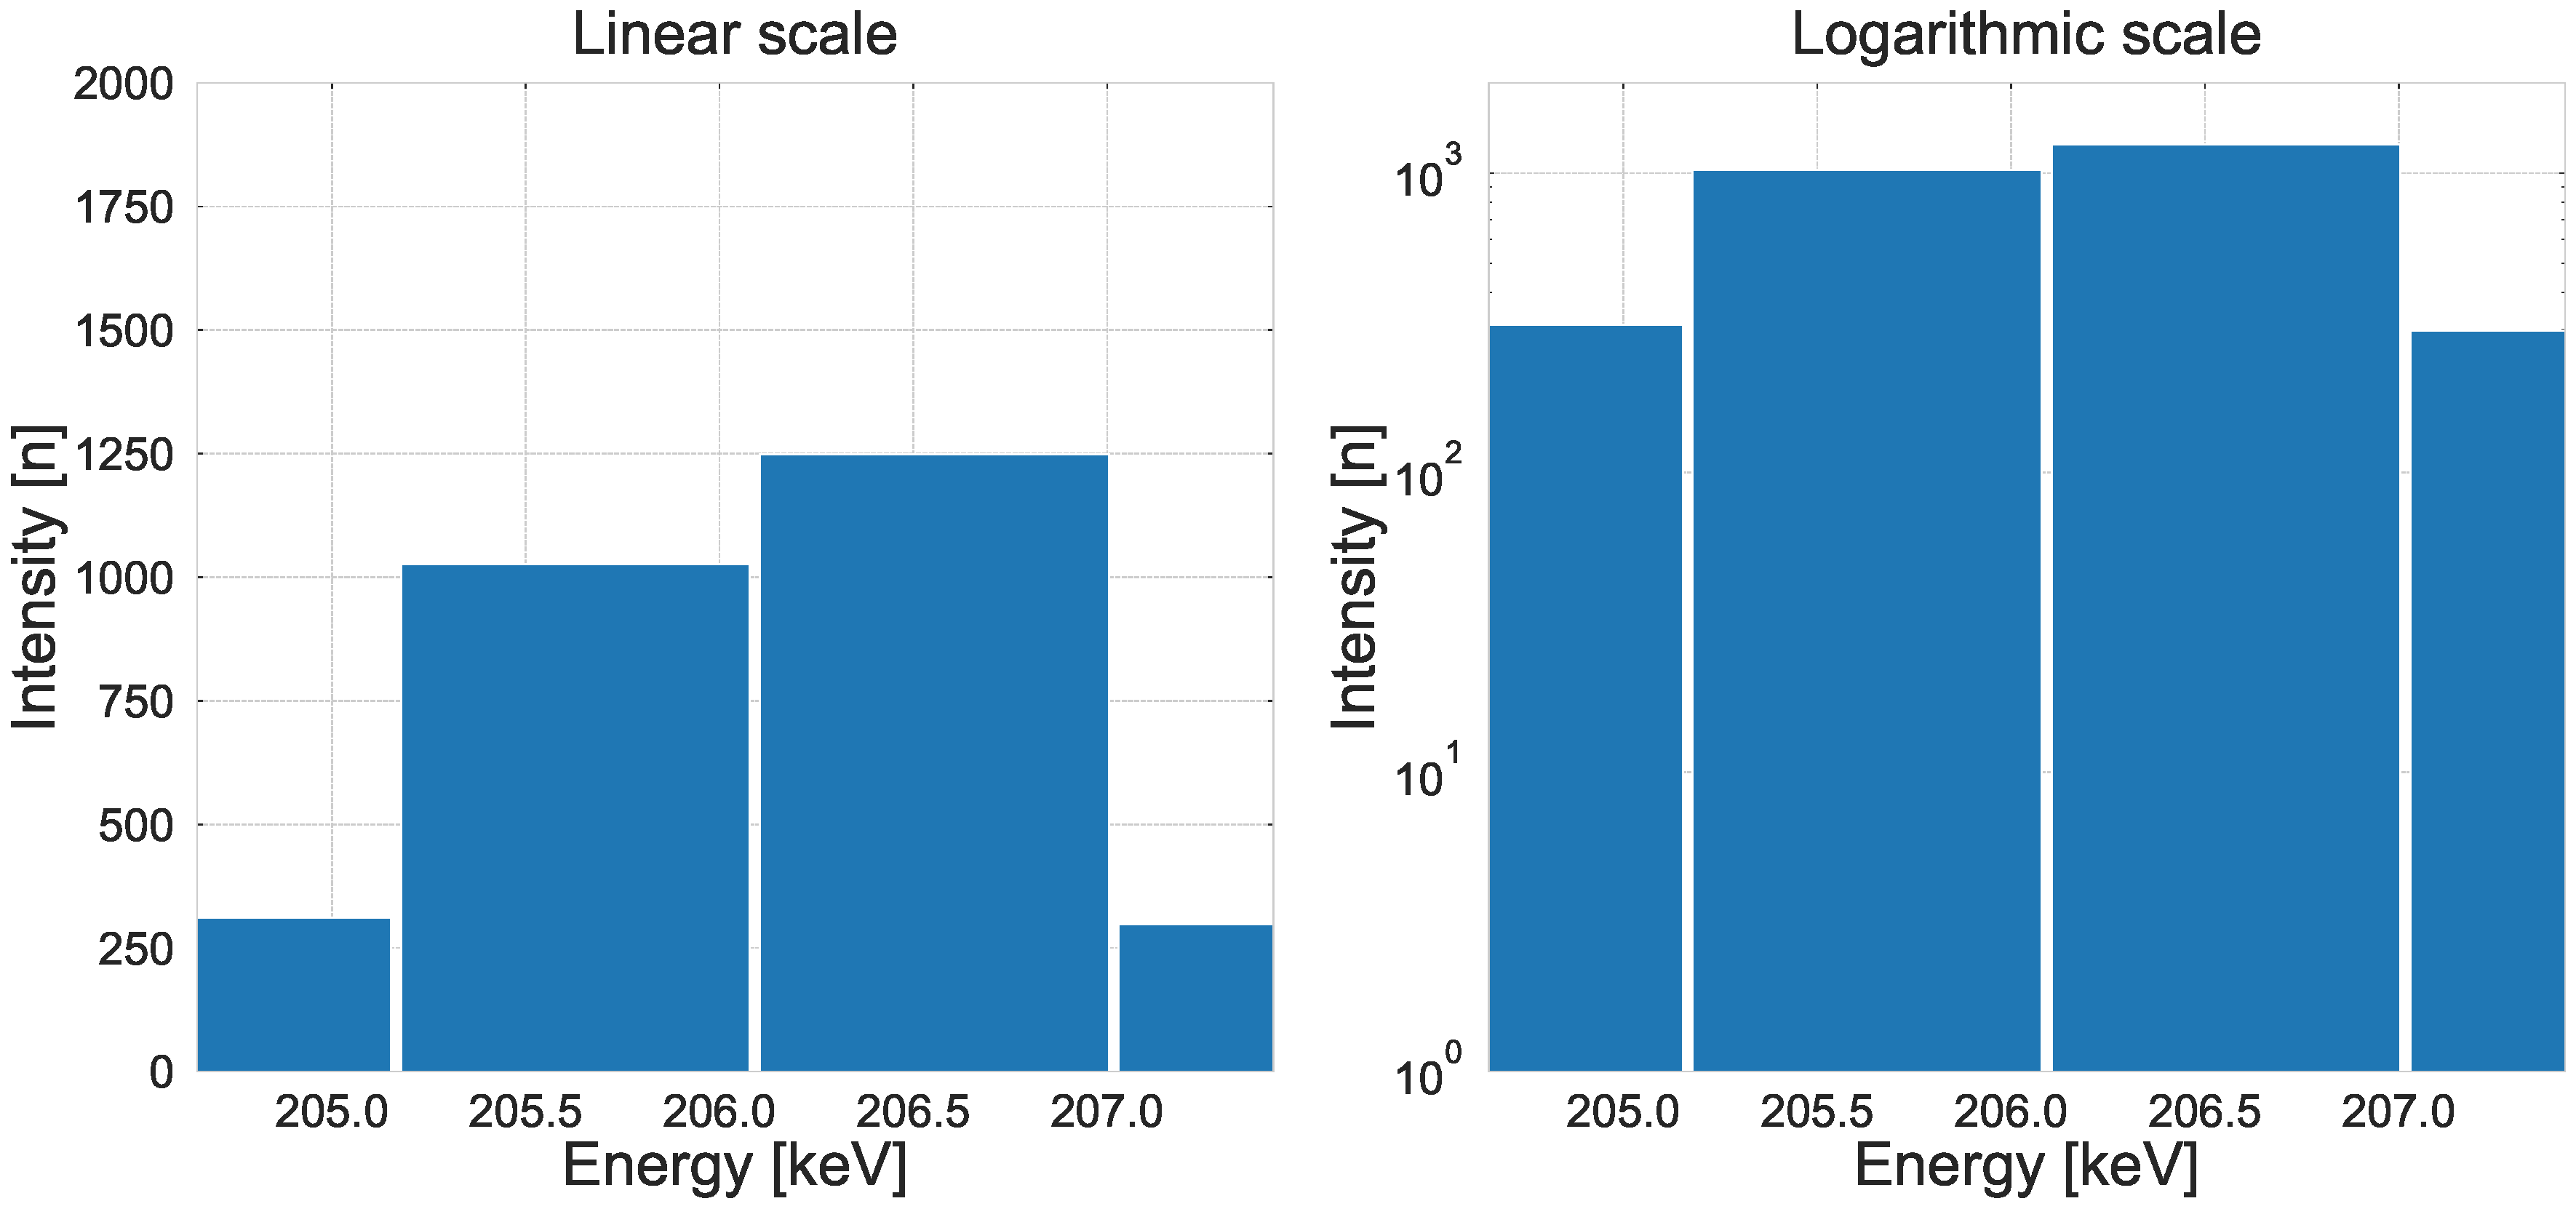
\includegraphics[width=\textwidth]{{images/spectra_lims_204.65_207.43_U235_g5_0}.pdf}
    \captionof{figure}{Az általam vizsgált anyag gamma-spektrumában található $^{235}$U, $\gamma_{5,0}$ tranziensből származó fotonjának foto-csúcsa.} \label{fig:7}
\end{center}
\begin{center}
    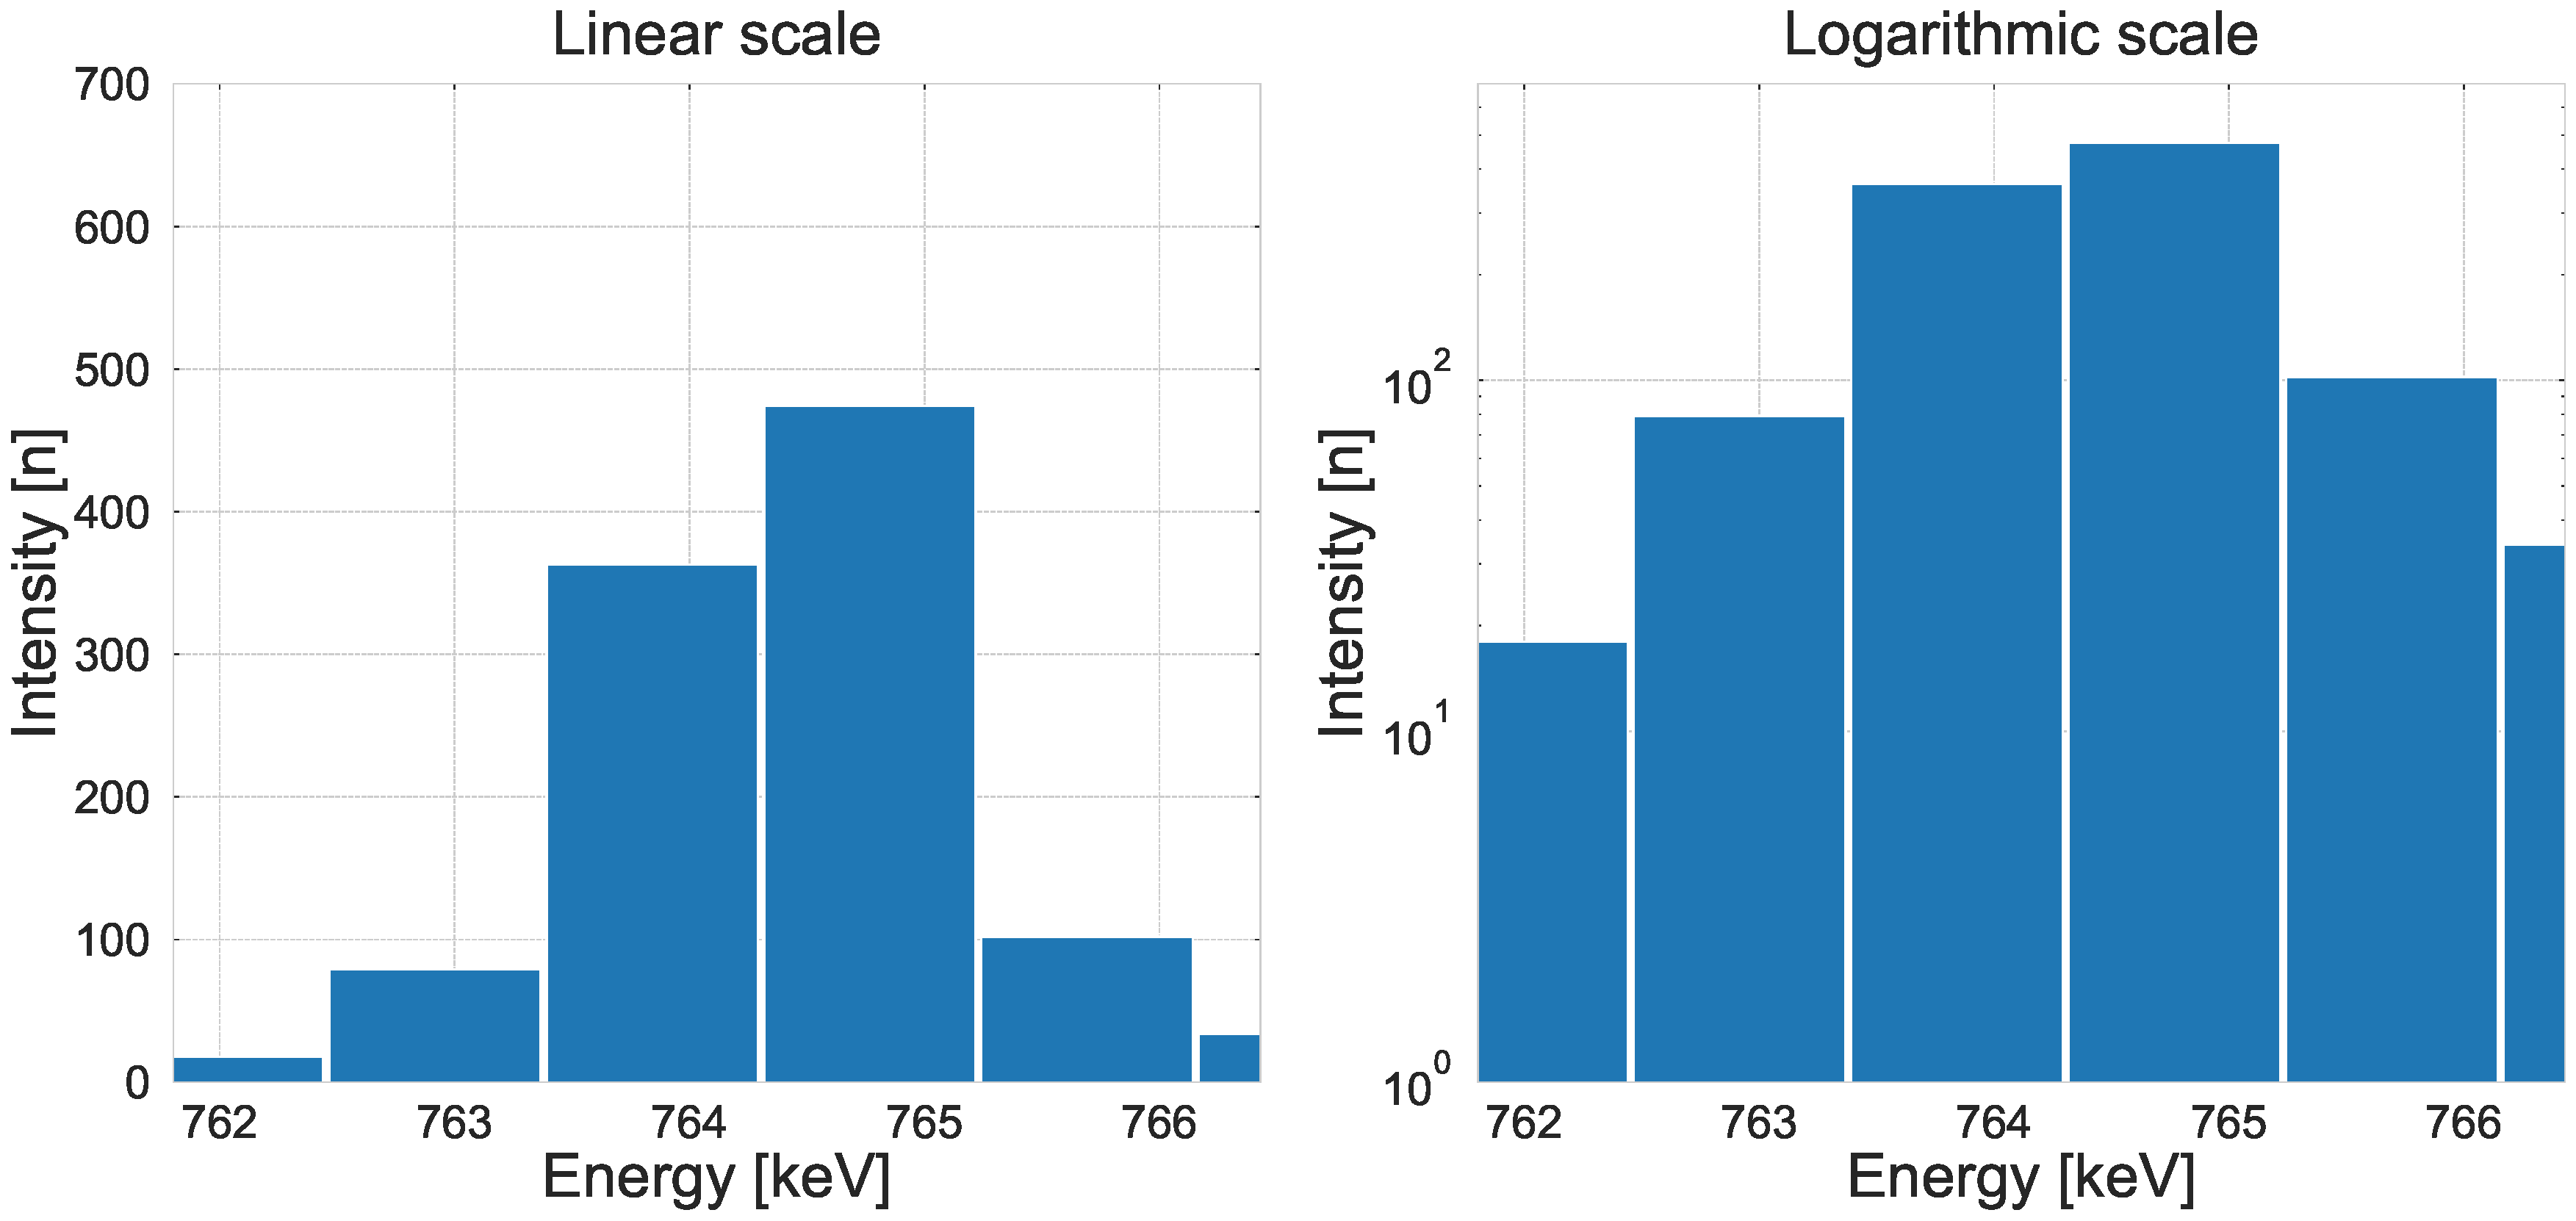
\includegraphics[width=\textwidth]{{images/spectra_lims_761.80_766.43_Unknown}.pdf}
    \captionof{figure}{Az általam vizsgált anyag gamma-spektrumában található ismeretlen eredetű foto-csúcs.} \label{fig:8}
\end{center}
\begin{center}
    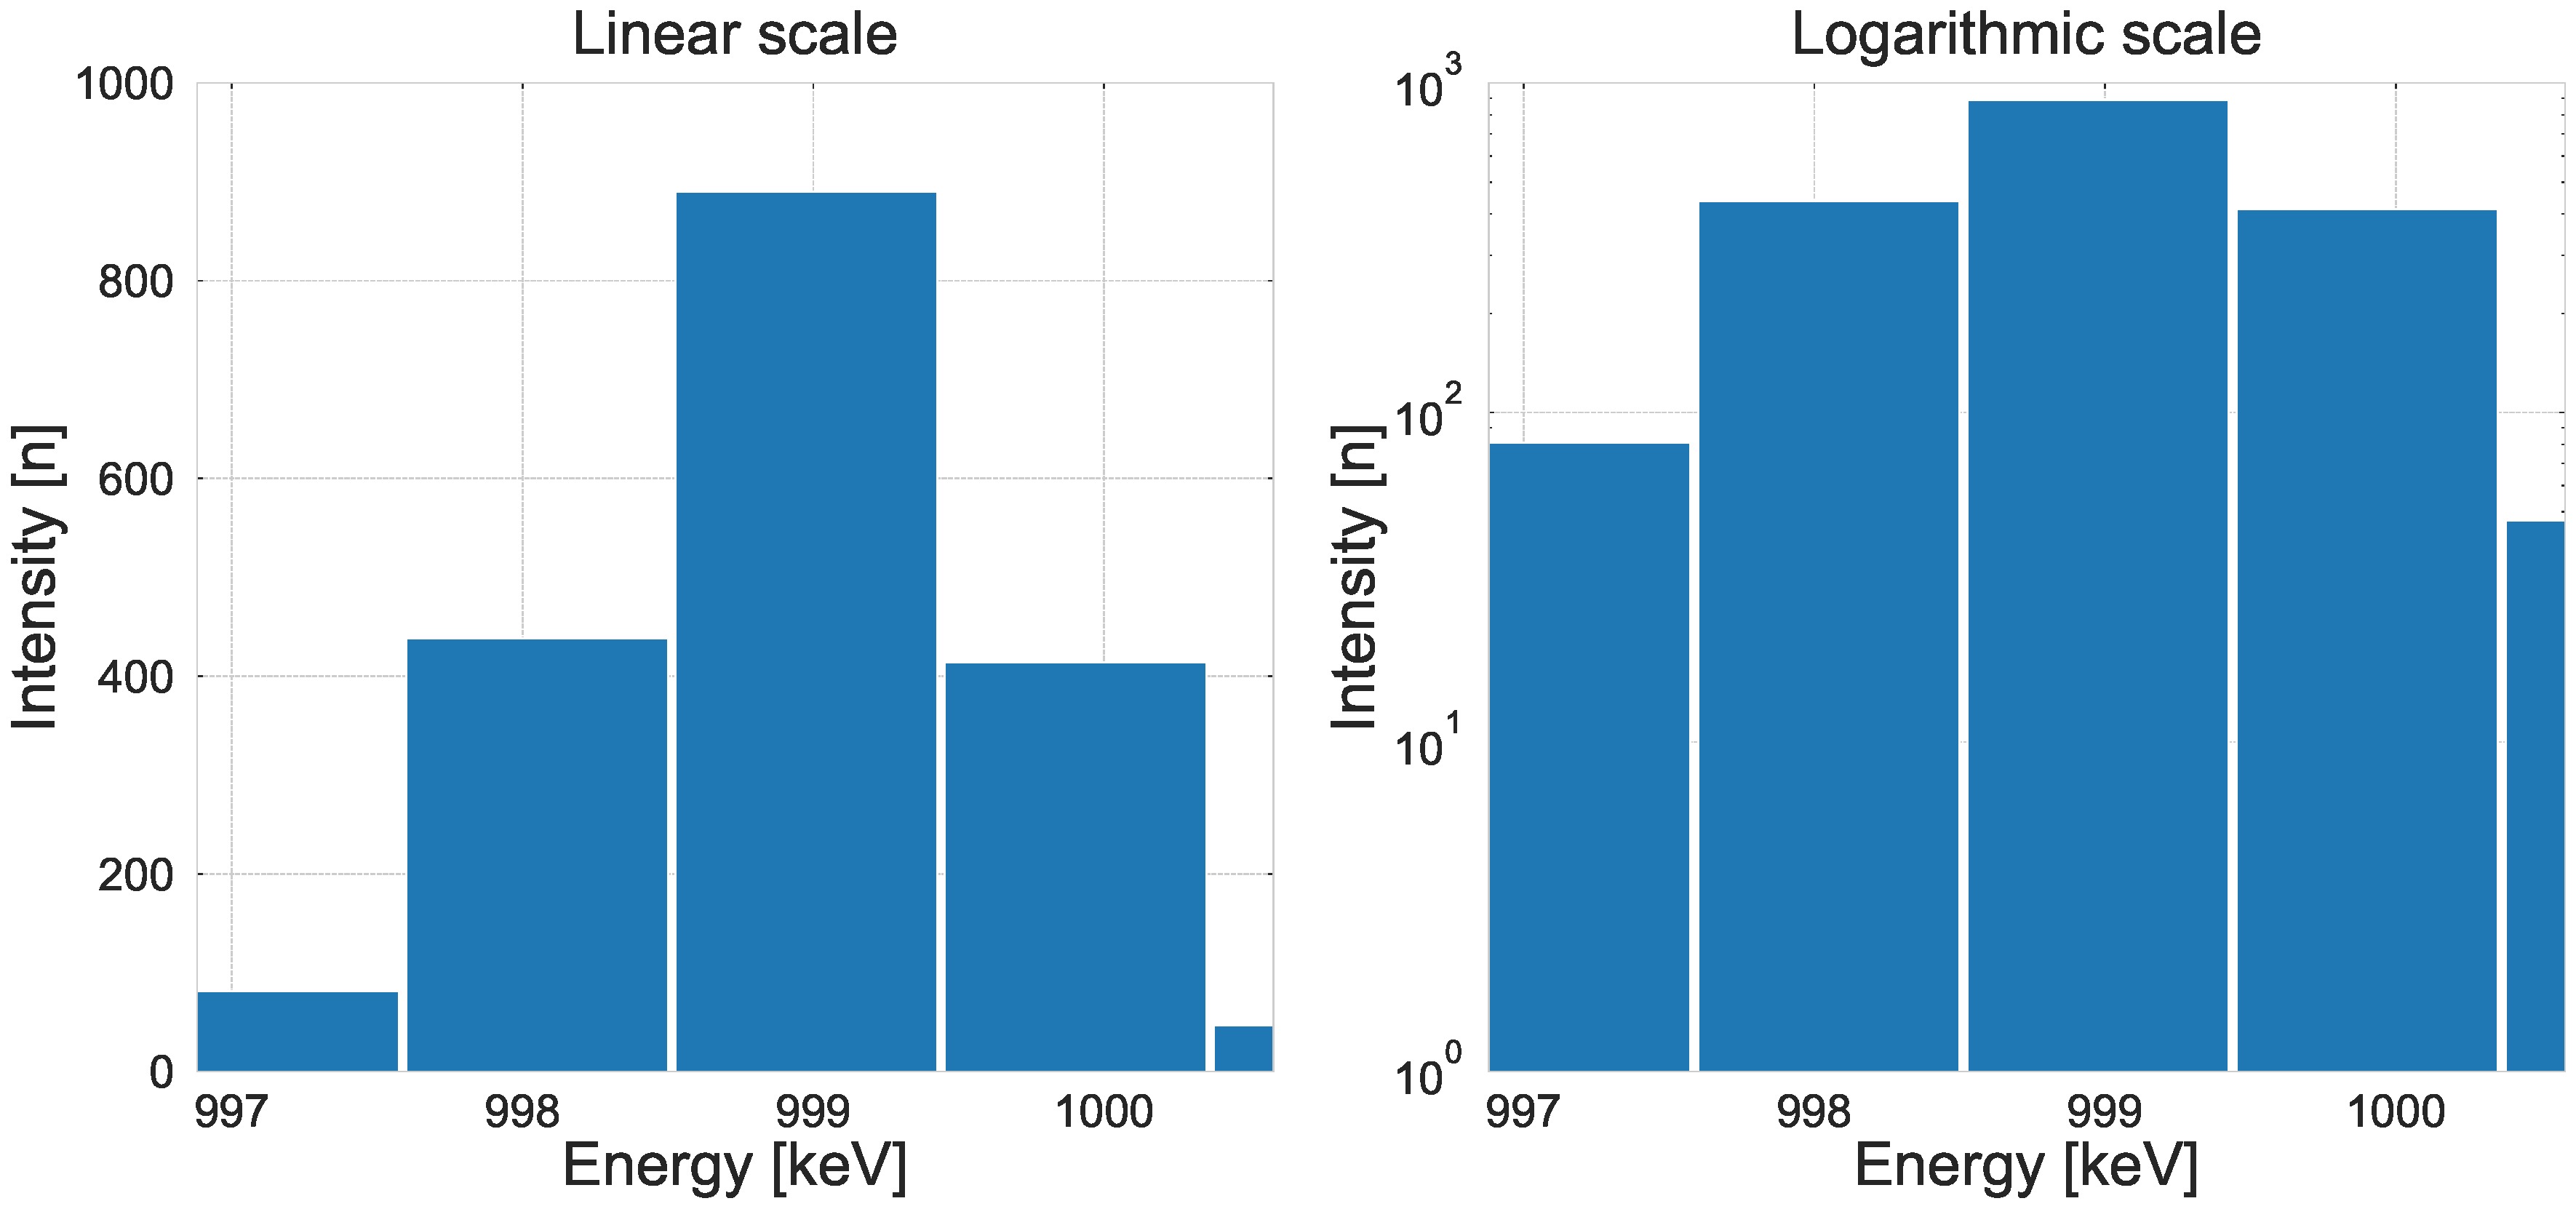
\includegraphics[width=\textwidth]{{images/spectra_lims_996.88_1000.58_Pam234_g9_1}.pdf}
    \captionof{figure}{Az általam vizsgált anyag gamma-spektrumában található $^{233}$Pa$^{m}$, $\gamma_{9,1}$ tranziensből származó fotonjának foto-csúcsa.} \label{fig:9}
\end{center}
\vspace*{\fill}

\section*{Appendix B - Táblázatok} \label{B}
\begin{center}
\begin{tabular}{|c|c|c|c|c|c|c|}
\hline
Izotóp 			 & Mért $E_{\gamma}$ (keV) & Valós $E_{\gamma}$ (keV)  & Intenzitás (\%) & Tranziens             & $S_{\text{csúcs}}$ & $\delta S_{\text{csúcs}}$ (\%) \\
\hline
$^{235}$U        & $145,28$       & $143,768$       & $13,20$          & $\gamma_{\text{4,1}}$ & $3375$  & $2,35$ \\
$^{235}$U  		 & $164,75$ 	  & $163,358$       & $5,855$          & $\gamma_{\text{5,1}}$ & $1976$  & $4,05$ \\
$^{235}$U  	     & $186,79$ 	  & $185,722$       & $63,41$          & $\gamma_{\text{4,0}}$ & $20836$ & $0,73$ \\
$^{235}$U  		 & $206,10$ 	  & $205,316$       & $5,465$          & $\gamma_{\text{5,0}}$ & $1666$  & $2,86$ \\
?                & $764,24$ 	  & ?    		    & ?    		       & ?                     & $1550$  & $2,16$ \\
$^{234}$Pa$^{m}$ & $998,77$ 	  & $1001,441$      & $8,56 * 10^{-1}$ & $\gamma_{\text{9,1}}$ & $914$   & $3,75$ \\
\hline
\end{tabular}
\captionof{table}{A gamma-spektrum kiértékelésekor vizsgált csúcsok adatai, $t = 1073$ s mérési idő és $N = 264077$ db detektált jel után (\cite{lnhb_235U} és \cite{lnhb_234Pa_m}).} \label{table:1}
\end{center}

\begin{center}
\begin{tabular}{|c|c|c|c|}
\hline
Izotóp 			 & $E_{\gamma}$ (keV) & Intenzitás (\%) & Felezési idő \\
\hline
$^{243}$Cm       & $760$     & $0$              & $29,1$ év    \\
$^{249}$Cf       & $760$     & $2 * 10^{-2}$    & $351$ év     \\
$^{150}$Eu       & $762,03$  & $2,8 * 10^{-2}$  & $36.9$ év    \\
$^{239}$Pu       & $763,61$  & $2.22 * 10^{-8}$ & $24110$ év   \\
$^{241}$Am       & $763,9$   & $2 * 10^{-7}$    & $432.2$ év   \\
$^{110}$Ag$^{m}$ & $763,944$ & $22,14$          & $249.79$ nap \\
$^{152}$Eu       & $764,900$ & $2,15 * 10^{-1}$ & $	13.537$ év \\
$^{160}$Tb       & $765,28$  & $2,140$          & $72.3$ nap   \\
$^{252}$Es       & $765,30$  & $1,83 * 10^{-1}$ & $471.7$ nap  \\
$^{192}$Ir       & $765,8$   & $1,49 * 10^{-3}$ & $73.831$ nap \\
\hline
\end{tabular}
\captionof{table}{A $764.24$ keV-es csúcsot okozható, $50$ napnál hosszabb felezési idejű magok listája \citep{lnbl_nuclear}} \label{table:2}
\end{center}

\begin{center}
\begin{tabular}{|c|c|c|c|}
\hline
Izotóp 			 & Mért $E_{\gamma}$ (keV) & $\eta$ (\%)          & $\delta \eta$ (\%) \\
\hline
$^{235}$U 		 & $145,28$                & $1,33059 * 10^{-1}$  & $2,218$            \\
$^{235}$U 		 & $164,75$ 	           & $1,23267 * 10^{-1}$  & $2,336$            \\
$^{235}$U 		 & $186,79$ 	           & $1,00812 * 10^{-1}$  & $3,085$            \\
$^{235}$U        & $206,10$ 	           & $1,06556 * 10^{-1}$  & $2,129$            \\
?                & $764,24$ 	           & $2,1255 * 10^{-2}$   & $2,16$             \\
$^{234}$Pa$^{m}$ & $998,77$ 	           & $2,7098 * 10^{-2}$   & $3,75$             \\
\hline
\end{tabular}
\captionof{table}{A detektor $\eta$ hatásfoka az egyes foto-csúcsok energiatartományaiban} \label{table:3}
\end{center}

\begin{center}
\begin{tabular}{|c|c|c|c|c|c|}
\hline
Izotóp 			 & $A$ (Bq) & $\delta A$ (\%) & $\lambda$ ($1/s$)   & $N$ (db)         & $\delta N$ (\%) \\
\hline
$^{235}$U 		 & $1.790$  & $0.046$ 		  & $3.12 * 10^{-17}$   & $5.74 * 10^{16}$ & $=\delta A$ \\
$^{235}$U 		 & $2.552$  & $0.064$ 		  & $3.12 * 10^{-17}$   & $8.18 * 10^{16}$ & $=\delta A$ \\
$^{235}$U 		 & $3.037$  & $0.038$ 		  & $3.12 * 10^{-17}$   & $9.74 * 10^{16}$ & $=\delta A$ \\
$^{235}$U        & $2.667$  & $0.050$ 		  & $3.12 * 10^{-17}$   & $8.55 * 10^{16}$ & $=\delta A$ \\
?                & ?        & $0.043$         & ?                   & ?                & $=\delta A$ \\
$^{234}$Pa$^{m}$ & $36.722$ & $0.074$ 		  & $4.92 * 10^{-18}$   & $7.46 * 10^{18}$ & $=\delta A$ \\
\hline
\end{tabular}
\captionof{table}{Az egyes foto-csúcsokhoz tartozó aktivitás értékek, bomlási állandól, valamit részecskeszámok és ezek hibái} \label{table:4}
\end{center}